% Modèles de calculabilité
% ========================

\chapter{Modèles de calculabilité}
\label{sec:mod_le_de_la_calculabilit_}

\section{Familles de modèles}
\label{sub:fammilles_de_mod_les}

Il y a deux grandes familles de modèles :
\begin{itemize}
	\item Modèle de calcul (calcule une réponse)
	\item Modèle de langages (décide l'appartenance à un ensemble)
\end{itemize}

\subsection{Modèles de calcul}
\label{ssub:mod_le_de_calcul}
L'objectif est de modéliser le concept de fonctions calculables, processus de
calcul, algorithme effectif.

On peut encore classer les modèles de calcul en 2 catégories, les
modèles déterministes et les modèles non déterministes.

\begin{mydef}[Modèles déterministes] une seule exécution possible
\end{mydef}

\begin{mydef}[Modèles non déterministes] il existe plusieurs exécutions
	possibles
\end{mydef}

On va voir les modèles de calcul suivant :
\begin{itemize}
	\item Automate fini
	\item Automate à pile
	\item Machine de Turing
	\item Langages de programmation
	\item Lambda calcul
	\item Fonction récursive
\end{itemize}
Mais il en existe beaucoup d'autres.
% subsubsection mod_le_de_calcul (end)

\subsection{Modèles de langage}
\label{ssub:mod_le_de_langage}
Un langage est défini pas une grammaire formelle. L'objectif est de modéliser
une classe de langages. Le langage est alors soit un ensemble récursif, soit un
ensemble récursivement énumérable.

% subsubsection mod_le_de_langage (end)
% subsection fammilles_de_mod_les (end)

\section{Langages de programmation}
\label{sub:langages_de_programmation}
C'est un modèle possible de la calculabilité. Pour définir un langage de
programmation comme modèle de la calculabilité, il faut définir :
\begin{itemize}
	\item Syntaxe du langage
	\item Sémantique du langage
	\item Convention de représentation d'une fonction par un programme
\end{itemize}

On se pose la question de savoir s'il y a des langages plus puissants que
d'autres. On va montrer que tous les langages complets sont équivalents. (Et la
plupart des langages sont complets.)

\paragraph{} Mais, il existe aussi des langages qui ne sont pas complets comme le
langage BLOOP (bounded loop).

\begin{mydef}
	BLOOP : Sous ensemble de Java qui ne calcule que des fonctions totales.
	(pas de boucle while, boucle for mais sans modification du compteur
	dans le for, pas de goto en arrière, pas de fonctions récursives)
\end{mydef}

BLOOP a donc toutes les propriétés qui découlent du chapitre précédent:

\begin{myprop}
Tous les programmes BLOOP se terminent :\\
    $ \Rightarrow$ BLOOP ne calcule que des fonctions totales\\
    $ \Rightarrow$ L'interpréteur est une fonction totale non calculable en
BLOOP (Hoare-Allison)\\
    $ \Rightarrow$ BLOOP ne calcule pas toutes les fonctions totales\\
    $ \Rightarrow$ BLOOP n'est pas un modèle complet de la calculabilité\\

Cependant il existe un compilateur des programmes BLOOP (Java).\\
\end{myprop}

% subsection langages_de_programmation (end)

\subsection{Langage de programmation non déterministe}
\label{ssub:langague_de_programmation_non_d_terministe}

\begin{myrem}
	Il est difficile d'avoir de l'intuition sur cette partie. On peut
	voir un programme ND comme un programme qui produit des résultats
	différents d'une exécution à l'autre. On peut représenter toutes
	les exécutions possibles du programmes sous forme de branches d'un
	arbre. Pour analyser la complexité, on ne
	considère que la profondeur de l'arbre (longueur de la branche
	la plus longue).
\end{myrem}

On va un introduire un nouveau langage ND-Java qui est le langage Java
auquel on ajoute le non-déterminisme sous la forme d'une fonction
prédéfinie $choose(n)$. Celle-ci retourne un entier compris entre $0$ et $n$ et elle
est non déterministe.

On peut voir un programme ND de 2 manières différentes :
\begin{enumerate}
	\item Il calcule une relation plutôt qu'une fonction
	\item C'est un moyen de décider si un élément appartient à un
		ensemble
\end{enumerate}
On considère l'approche 2 en calculabilité.

\begin{mydef}[ND-récursif] \label{def:ND-rec}
	Un ensemble $A \subseteq \N$ est ND-récursif s’il existe un
	ND-programme tel que lorsqu'il reçoit comme donnée n'importe quel nombre
	naturel $x$ \\
	\begin{tabular}{l}
	si $x \in A$ alors il existe une exécution fournissant tôt ou tard
	comme résultat 1 \\
	si $x \notin A$ alors toutes les exécutions fournissent tôt ou tard
	comme résultat 0 \\
	\end{tabular}
\end{mydef}

\begin{mydef}[ND-récursivement énumérable] \label{def:ND-recenum}
	Un ensemble $A \subseteq \N$ est ND-récursivement énumérable s’il existe un
	ND-programme tel que lorsqu'il reçoit comme donnée n'importe quel nombre
	naturel $x$ \\
	\begin{tabular}{l}
	si $x \in A$ alors il existe une exécution fournissant tôt ou tard
	comme résultat 1 \\
	si $x \notin A$ alors les exécutions possibles ne se terminent pas ou
	retournent un résultat $\neq 1$ \\
	\end{tabular}
\end{mydef}

\begin{myprop} \label{prop:ND-eq}
	On peut simuler les exécutions d'un ND-programme à l'aide d'un programme
	déterministe.
	\begin{proof}
		Soit un programme non-déterministe quelconque à N branches (N \textit{threads}).
		Montrons qu'on peut construire un programme déterministe équivalent.
		Il suffit de créer un programme qui exécute séquentiellement chacune des N branches de l'arbre.
		Cependant les branches pouvant être infinies, il est nécessaire d'explorer ces branches de l'\ arbre d'exécution en largeur d'abord (\textit{Breadth First Search}). La complexité temporelle du programme ainsi construit devient exponentielle.  En effet, un arbre de profondeur $k$ a un nombre exponentiel de noeuds.
	\end{proof}
\end{myprop}

\paragraph{Exemple} : Le ND-programme à gauche (figure \ref{fig:ND_tree}) comporte 3 branches et  a une hauteur de 3. Il est tranformé en un programme D, à droite (fiure \ref{fig:D_tree}) qui a une longueur de 9. \\
	\input{Images/ND_to_D_Exemple.tex}

\begin{myprop}
	Un ensemble est ND-récursif ssi il est récursif
	\begin{proof}
		Si un ensemble A quelconque est ND-récursif, alors il est récursif.
		En effet, s'il est ND-récursif, il existe un ND-programme qui permet de décider l'ensemble A (voir définition \ref{def:ND-rec}).
		Par la propriété \ref{prop:ND-eq}, on sait qu'il existe alors un programme déterministe équivalent qui décide A. À ce programme correspond un algorithme.
		Selon la définition \ref{def:recursif}, l'ensemble A est alors récursif.

		Inversement, si un ensemble A quelconque est récursif, alors il est ND-récursif. En effet, par définition, il existe un programme D qui décide A.
		Ce programme peut être vu comme un programme ND avec seulement une branche. A est donc également ND-récursif.
	\end{proof}
\end{myprop}

\begin{myprop}
	Un ensemble est ND-récursivement énumérable ssi il est récursivement énumérable
	\begin{proof}
		Si un ensemble A quelconque est ND-récursivement énumérable, alors il est récursivement
		énumérable.
		En effet, s'il est ND-récursivement énumérable, il existe un ND-programme dont le comportement est décrit à la définition \ref{def:ND-recenum}.
		Par la propriété \ref{prop:ND-eq}, on sait qu'il existe alors un programme déterministe qui se comporte de manière équivalente. À ce programme correspond un algorithme.
		Selon la définition \ref{def:recursivement enum}, l'ensemble A est alors récursivement énumérable.

		Inversement, si un ensemble A quelconque est récursivement énumérable, alors il est ND-récursivement énumérable. En effet, par définition, il existe un programme D qui se comporte comme décrit dans la définition \ref{def:recursivement enum}.
		Ce programme peut être vu comme un programme ND avec seulement une branche. A est donc également ND-récursivement énumérable.
	\end{proof}

\end{myprop}

\section{Automates finis FA}
\label{sub:automates_finis}

\paragraph{Objectif :} Décider si un mot donné appartient ou non à un langage.

\paragraph{Utilisation :} Utilisé dans les interfaces pour les humains (par
exemple, les distributeurs).

\subsection{Modèles des automates finis}
\label{ssub:mod_les_des_automates_finis}
Un automate fini est composé de :

\begin{itemize}
	\item $\Sigma$ : ensemble fini de symboles
	\item $S$ : ensemble fini d'états
	\item $s_0 \in S$ : état initial
	\item $A \subseteq S$ : ensemble des états acceptants
	\item $\delta: S \times \Sigma \rightarrow S$ : fonction de transition
\end{itemize}


\paragraph{Fonctionnement}
\begin{itemize}
	\item départ avec un état initial
	\item parcours des symboles du mot d'entrée, un à un
	\item à chaque symbole lu, l'état change (fonction de transition
		$\delta$) en fonction de l'état courant et du symbole lu
	\item l'état final est l'état après avoir parcouru tous les symboles en
		entrée
	\item l'état final peut-être acceptant ou non
\end{itemize}

\begin{myrem}
	Il n'y a donc pas de mémoire. De plus, un automate peut-être simulé
	par un programme Java.
\end{myrem}

\begin{myprop}
	Un automate fini définit un ensemble récursif de mots $=\{m \ |\ m$ est
		accepté par FA$\}$
\end{myprop}

\begin{myprop}
	Certains ensembles récursifs ne peuvent pas être reconnus par un
	automate fini. Par exemple $L = \{ a^n b^n \ | \ n\geq 0\}$ (parce qu'il nécessiterait un nombre infini d'états)
\end{myprop}

\begin{myprop}
	L'interpréteur des automates finis est calculable, mais ne peut pas être
	représenté par un automate fini, car ce n'est pas un \textbf{modèle
	complet} de la calculabilité (Hoare-Allison)
\end{myprop}

\begin{mydef}[Langage régulier] Un langage régulier est un langage défini par une expression
	régulière.
\end{mydef}

\paragraph{Exemple}
Un exemple simple de mécanisme qui peux être modélisé par un automate fini est le portillon d'accès. Dans le métro par exemple, lorsqu'un ticket est inséré, le portillon se déverrouille et le passage d'un usagé est autorisé, lorsque celui ci est passé, il se verrouille à nouveau. Le portillon peut être modélisé comme un automate fini comportant deux états: verrouillés et déverrouillé. L'état peut-être modifié par l'ajout d'un ticket/jeton (entrée: jeton). Soit lorsque l'utilisateur pousse les barres du portillon (entrée: pousser). La fonction de transition est représentée par la table \ref{FTPortillon}. La figure \ref{diagrammeetat} illustre le diagramme d'état de cet automate.

\begin{figure}[h]
	\centering
	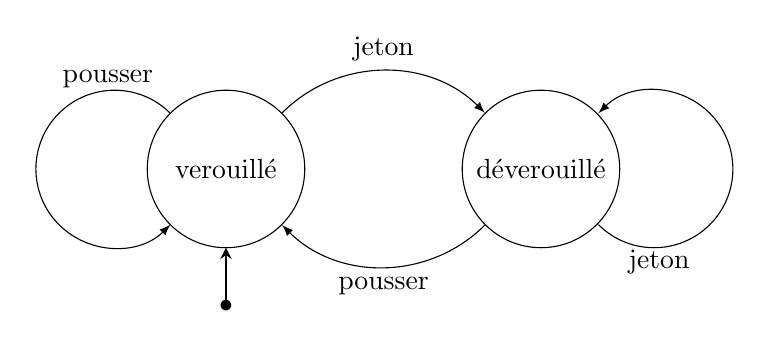
\begin{tikzpicture}
		\node[draw,minimum height=2cm,circle] (A) at (0,0) {verouillé};
		\node[draw,minimum height=2cm,circle] (B) at (4,0) {déverouillé};
		\draw (0,-1.75) node {$\bullet$};
		
		\draw[->,>=stealth,thick] (0,-1.75) -- (0,-1);
		
		\draw[->,>=latex] (A) to[out=45,in=135] (B);
		\draw[->,>=latex] (B) to[out=-135,in=-45] (A);
		\draw[->,>=latex] (-0.7071,0.7071) arc(45:315:1);
		\draw[->,>=latex] (4.73,-0.7071) arc(-135:135:1);
		
		\draw (-1.5,0.9) node[above] {pousser};
		\draw (2,-1.25) node[below] {pousser};
		\draw (2,1.25) node[above] {jeton};
		\draw (5.5,-0.9) node[below] {jeton};
	\end{tikzpicture}
	\caption{Diagramme d'état du portillon \\{\footnotesize
			Par ManiacParisien — Travail personnel, CC BY-SA 4.0, https://commons.wikimedia.org/w/index.php?curid=47664521}}
	\label{diagrammeetat}
\end{figure}


\begin{table}[h]
	\centering
	
	\begin{tabular}{|l|l|l|}
		\hline
		& Pousser    & Jeton       \\ \hline
		Verrouillé   & Verrouillé & Déverrouillé \\ \hline
		Déverrouillé & Verrouillé & Déverrouillé \\ \hline
	\end{tabular}
	\caption{Fonction de transition du portillon}
	\label{FTPortillon}
\end{table}  

Un exemple plus complexe est le célèbre problème du passeur. Celui ci doit traverser une rivière, avec un loup, une salade et une chèvre. Dans sa barque il ne peut prendre qu'un objet avec lui. La difficulté supplémentaire est que la chèvre et le loup ne peuvent pas rester ensemble et la chèvre ne peut pas rester seule avec la salade. Chaque état représente les objets se trouvant sur l'autre rive, P étant le passeur, C la chèvre, L le loup et S la salade. Sur les flèches, la lettre correspond à l'objet transporté avec lui lors de la traversée. Au début rien n'a été transporté, à la fin, les trois objets et le passeur se retrouvent sur l'autre rive.
La figure \ref{Salade} illustre le diagramme d'état de cette énigme.
\begin{figure}[h]
	\centering
        % Ne pas utiliser le fichier Images/567px-ChevreLoupSalade.jpg car travis n'arrive pas à builder avec cette version
	\includegraphics[width=0.4\textwidth]{Images/ChevreLoupSalade.jpg}
	\caption{Diagramme d'état du passeur \\{\footnotesize Par ManiacParisien — Travail personnel, CC BY-SA 4.0, https://commons.wikimedia.org/w/index.php?curid=47815891}}
	\label{Salade}
\end{figure}

Un autre exemple d'automate fini est un distributeur de boissons qui reçoit une pièce d'argent et un choix de boisson puis sert la boisson choisie. Par exemple, nous pouvons considérer que la machine reçoit une pièce de 2 euros et a uniquement trois choix Fanta, Coca, Eau. Un tel système peut être modélisé comme suit:\\

\begin{figure}
	\centering
	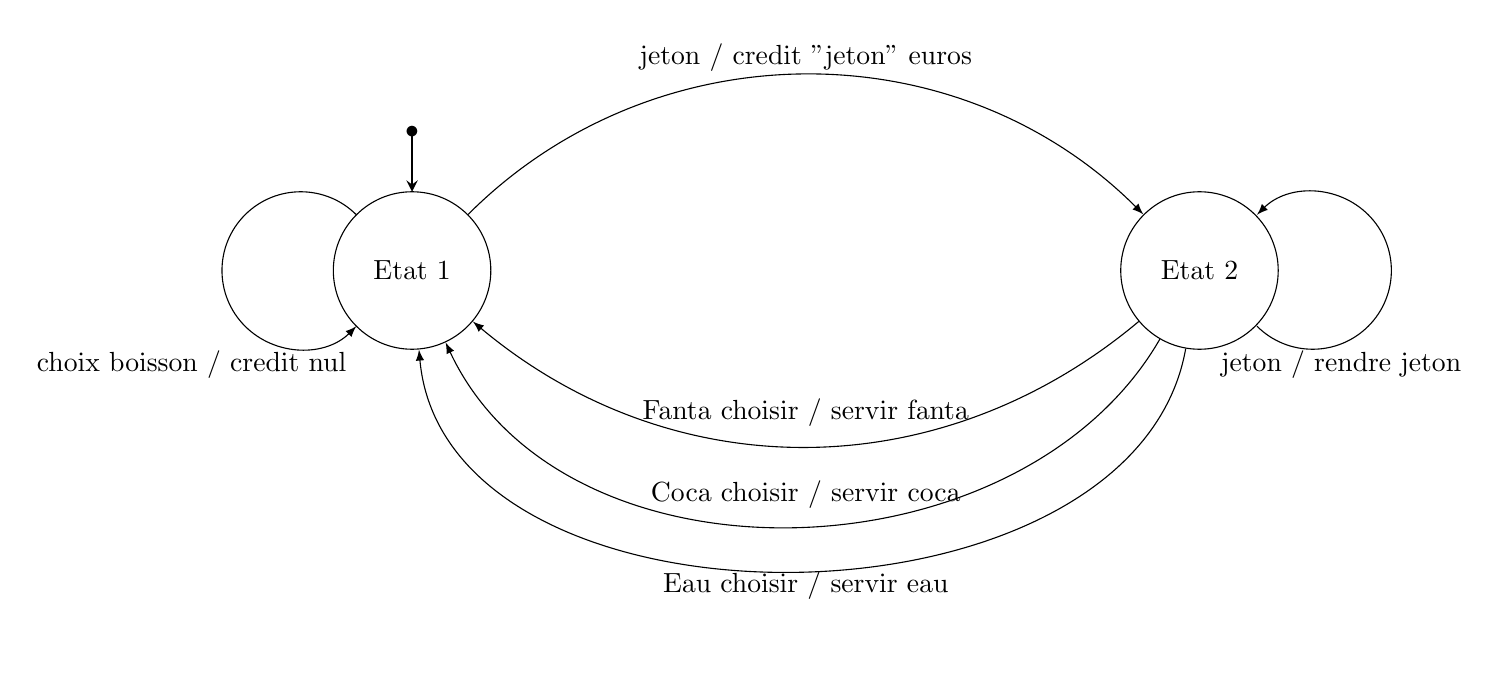
\begin{tikzpicture}
		\node[draw,minimum height=2cm,circle] (A) at (0,0) {Etat 1};
		\node[draw,minimum height=2cm,circle] (B) at (10,0) {Etat 2};
		\draw (0,1.75) node {$\bullet$};
        
        \draw[->,>=stealth,thick] (0,1.75) -- (0,1);
		
		\draw[->,>=latex] (A) to[out=45,  in=135] (B);
		
		\draw[->,>=latex] (B) to[out=-140, in=-40] (A);
		\draw[->,>=latex] (B) to[out=-120, in=-65] (A);
		\draw[->,>=latex] (B) to[out=-100, in=-85] (A);
		
        \draw[->,>=latex] (-0.7071,0.7071) arc(45:315:1);
        \draw[->,>=latex] (10.73,-0.7071) arc(-135:135:1);
		
		\draw (5,-1.50) node[below]  {Fanta choisir / servir fanta};
		\draw (5,-2.55) node[below]  {Coca choisir / servir coca};
		\draw (5,-3.70) node[below] {Eau choisir / servir eau};
		
		\draw (5,2.40) node[above] {jeton / credit "jeton" euros};
		
		\draw (11.8,-0.9) node[below] {jeton / rendre jeton};
		
		\draw (-2.8,-0.9) node[below] {choix boisson / credit nul};


	\end{tikzpicture}
	\caption{Diagramme d'état d'un distributeur de boisson simple \\{Inspirer du TD7 : Automates Par Stephane Devismes Université Grenoble Alpes}}
\end{figure}
Les transitions avec les mêmes états de départs et d’arrivées et la même sortie ont une seule flèche étiquetée avec l’entrée / la sortie. 

\paragraph{Propriétés}
\begin{myprop}
	Un automate fini définit un ensemble récursif de mots $=\{m \ |\ m$ est
		accepté par FA$\}$.
\end{myprop}

\begin{myprop}
	Certains ensembles récursifs ne peuvent pas être reconnus par un
	automate fini.

    \begin{proof}
    Par exemple $L = \{ a^n b^n \mid n\geq 0\}$ : l'automate doit compter le nombre de $a$ pour vérifier qu'il y a autant de $b$. Mais il n'a pas de mémoire, donc pas de moyen de retenir le nombre $n$.

    Par contre, un automate fini pourrait reconnaître l'ensemble $L' = \{a^n b^m \mid n,m\geq 0\}$.
    \end{proof}
\end{myprop}

\begin{myprop}
	L'interpréteur des automates finis est calculable, mais ne peut pas être
	représenté par un automate fini, car ce n'est pas un \textbf{modèle
	complet} de la calculabilité (Hoare-Allison).
\end{myprop}

\begin{mydef}[Langage régulier] est un langage défini par une expression
	régulière.
\end{mydef}

\begin{mydef}[Expression régulière]
       	Dans le cours, la syntaxe d'une expression régulière est la suivante :
	\begin{description}
		\item[+] ou
		\item[.] concaténation
		\item[*] fermeture de Kleene\footnote{définit un groupe qui existe zéro, une ou plusieurs fois}
		\item[( )] répétition
	\end{description}
\end{mydef}


% subsubsection mod_les_des_automates_finis (end)

\subsection{Extension des automates finis}
\label{ssub:automate_fini_nd}
\paragraph{NDFA} On étend le modèle en permettant d'avoir plusieurs transitions possibles pour
une paire <état,symbole>. Ce qui implique que plusieurs exécutions sont
possibles. On a donc plus une fonction de transition mais une relation de transition.

\paragraph{} De même, pour un ND programme, un mot est accepté par un NDFA
s'il existe au moins une exécution où l'état final est acceptant. Dans l'autre
sens, un mot n'est pas accepté si aucune exécution ne se termine avec l'état final
acceptant.

\begin{myprop}
	Si un ensemble récursif est défini par un NDFA, alors cet ensemble est
	défini par un FA.
\end{myprop}

\begin{myprop}
	Un NDFA définit un ensemble récursif de mots.
\end{myprop}

\paragraph{Ajout de transitions vides $\epsilon$} On peut encore étendre le modèle NDFA en
rajoutant une possibilité de transition sans lire de symbole (transition
spontanée). Ça a la même puissance et les mêmes propriétés qu'un NDFA.

% subsubsection automate_fini_nd (end)

\section{Automate à pile PDA}
\label{sub:automate_pile}
C'est une extension du modèle des automates finis. On ajoute une mémoire avec
la pile de symboles.
Les différences principales sont :
\begin{itemize}
	\item la transition entre états dépend du symbole lu et du symbole au
		sommet de la pile
	\item	chaque transition peut enlever le sommet de la pile et empiler
		de nouveaux éléments ou ne pas changer la pile.
\end{itemize}

\paragraph{Objectif :} Décider si le mot donné appartient ou non à un langage.

\paragraph{Utilisation :} Utilisé dans les compilateurs.

\paragraph{Composition :}
On rajoute $\Gamma$ et on change la fonction de transition en une nouvelle
relation de transition.
\begin{itemize}
	\item $\Sigma$ : ensemble fini de symboles d'entrée
	\item $\Gamma$ : ensemble fini de symboles de pile
	\item $S$ : ensemble fini d'états
	\item $s_0 \in S$ : état initial
	\item $A \subseteq S$ : ensemble des états acceptants
	\item $\Delta \subset S \times \Sigma \times \Gamma \rightarrow S \times
		\Gamma^*$ : relation de transition (finie)
\end{itemize}

\begin{myprop}
	Tout comme un NDFA, un PDA définit un ensemble récursif de mots (langage
	récursif).
\end{myprop}

\paragraph{Convention :}
\begin{itemize}
	\item Z est le symbole initial de la pile (pile vide)
	\item $\epsilon$ signifie qu’aucun symbole ne doit être lu pour cette
		transition (symbole ``vide'')
	\item A, B / C : A est le symbole lu, B est le symbole au
		sommet de la pile et C est ce qui va remplacer le
		sommet de la pile (peut-être un xB pour
		rajouter x sur la pile, $\epsilon$ pour retirer B du sommet de la pile,
		ou juste B pour ne pas changer le sommet)
\end{itemize}

\begin{myprop}
	Certains ensembles récursifs ne peuvent pas être reconnus par un automate
	à pile.
\end{myprop}

\begin{proof}
	Par exemple $\{a^n b^n a^n | n\geq 1\}$ : notre automate doit d'abord retenir le nombre $n$ dans la première série de $a$, puis vérifier qu'il y a bien $n$ occurrences de $b$ puis $n$ occurrences de $a$ dans la deuxième série. Le seul moyen de retenir $n$ est d'empiler un symbole dans la pile chaque fois qu'on lit un $a$, de sorte à avoir $n$ symboles empilés après la première série de $a$.

	Ensuite, on enlève un symbole chaque fois qu'on lit un $b$, sachant qu'on doit arriver au bout de la série de $b$ en même temps qu'on arrive au fond de la pile. Mais impossible alors de savoir combien d'occurrence de $a$ il faut compter dans la deuxième série de $a$, on ne connaît plus le nombre $n$ !
\end{proof}

\begin{myprop}
	Les automates à pile sont plus puissants que les automates finis (ils
	peuvent reconnaitre plus d'ensembles)
\end{myprop}

\begin{myprop}
	Ce n'est pas un modèle complet de la calculabilité donc par Hoare-
	Allison, l'interpréteur n'est pas calculable dans le modèle.
	% Lena : pas sûre du sens de l'implication
\end{myprop}

% subsection automate_pile (end)

\section{Grammaires et modèles de calcul}
\label{sub:grammaires_et_mod_les_de_calcul}

\paragraph{Objectif :}
Définition d'un langage (ensemble de mots) et à partir de la grammaire on peut
générer/dériver les mots du langage.

\paragraph{Utilisation :} Utilisé pour la définition de langages de
programmation, pour l'analyse du langage naturel...

\paragraph{Composition du modèle :}

\begin{itemize}
	\item $\Sigma$ : alphabet
	\item les éléments de $\Sigma$ sont des symboles terminaux
	\item autres symboles utilisés durant la dérivation : symboles non
		terminaux (A,B, ..., <dig>,..)
	\item S : point de départ de la dérivation (symbole non terminal)
\end{itemize}

\begin{mydef}[Règle de production]
	On appelle un ensemble de règles de dérivation des règles de production.
\end{mydef}

\begin{myexem}
	\begin{itemize}
		\item $\Sigma ={0,1,2}$
		\item $S \rightarrow <Dig>$
		\item $<Dig> \rightarrow D$
		\item $D \rightarrow 0 | 1 |2 | \epsilon $ ($\epsilon$ signifie rien)
	\end{itemize}
\end{myexem}

\begin{myexem}[Grammaire des réels dans Java]
$\Sigma =\{0,1,2,3,4,5,6,7,8,9,.,E\}$ avec les règles de production suivantes :
\begin{itemize}
\item $S\ \rightarrow\ <Real>$
\item $<Real>\ \rightarrow\ <Sig><Dig>.<Dig>$
\item $<Real>\ \rightarrow\ <Sig><Dig>.<Dig>E<Exp>$
\item $<Real>\ \rightarrow\ <Sig><Dig>E<Exp>$
\item $<Sig>\ \rightarrow\ \epsilon\mid +\mid -$
\item $<Dig>\ \rightarrow\ D$
\item $<Dig>\ \rightarrow\ D<Dig>$
\item $D\ \rightarrow\ 0\mid 1\mid 2\mid 3\mid 4\mid 5\mid 6\mid 7\mid 8\mid 9\mid$
\item $<Exp>\ \rightarrow\ <Dig>$
\end{itemize}
Par exemple, le réel $+3.14$ est dérivé comme suit (leftmost derivation) :
\begin{align*}
S\ &\rightarrow\ <Real>\\
&\rightarrow\ <Sig><Dig>.<Dig>\\
&\rightarrow\ +<Dig>.<Dig>\\
&\rightarrow\ +D.<Dig>\\
&\rightarrow\ +3.<Dig>\\
&\rightarrow\ +3.D<Dig>\\
&\rightarrow\ +3.1<Dig>\\
&\rightarrow\ +3.1D\\
&\rightarrow\ +3.14
\end{align*}
Ce même exemple peut être représenté par un arbre syntaxique :
\begin{center}
\begin{tikzpicture}[level distance=1.2cm,
  level 1/.style={sibling distance=3cm},
  level 2/.style={sibling distance=1.5cm}]
  \node {S}
    child {node {Real}
      child {node {Sig}
      	child {node {+}}
      }
      child {node {Dig}
      	child {node {D}
          child {node {3}}
        }
      }
      child {node {.}}
      child {node {Dig}
      	child {node {D}
       	  child {node {1}}
        }
        child {node {Dig}
          child {node {D}
          	child {node {4}}
          }
        }
      }
    };
\end{tikzpicture}
\end{center}
\end{myexem}

\begin{mydef}[Dériver] Appliquer des règles de la grammaire pour vérifier
	si une chaîne de symbole appartient au langage (on part d'une chaîne de symboles
	et on vérifie les règles sur celle-ci).
\end{mydef}

\begin{mydef}[Inférer] Dérivation dans ``le sens contraire'',
	c'est-à-dire, on part des règles de grammaire et on génère une chaîne
	de symboles.
\end{mydef}

\begin{mydef}[Arbre syntaxique]
	Un arbre syntaxique permet de représenter la dérivation, chaque noeud
	correspond à un symbole terminal ou non. Les arêtes correspondent à
	l'application d'une règle. Il y a plusieurs nœuds enfants si la règle
	``génère'' plusieurs symboles.
\end{mydef}

\begin{myprop}
	On peut dériver de plusieurs façons équivalentes, leftmost (on dérive
	toujours le plus à gauche d'abord), rightmost (contraire de leftmost)
	ou  aucun des deux.
\end{myprop}

\subsection{Hiérarchie de Chomsky}
\label{ssub:hi_rarchie_de_chomsky}

Chomsky a défini 4 types de grammaires formelles. On peut les classer selon
leur ``puissance''.

\begin{mydef}[Puissance d'une grammaire]
	Une grammaire A est plus puissante qu'une grammaire B si on peut définir plus
	de langages avec A qu'avec B.
\end{mydef}

On peut aussi faire correspondre chaque type de grammaire avec un type de
calcul permettant de reconnaitre un langage de cette grammaire.

\begin{tabular}{|c|c|c|}
	\hline
	 Type & Type de grammaire & Modèle de calcul\\
	 \hline
	3 & régulière & Automate fini \\
	 \hline
	2 & hors contexte & Automate à pile \\
	 \hline
	1 & sensible au contexte & Machine de Turing à ruban fini \\
	 \hline
	0 & récursivement énumérable & Machine de Turing \\
	\hline
\end{tabular}

Chaque type de grammaire est défini par une règle de production A $\rightarrow
$ B. Il y a des conditions différentes sur A et B selon le type de
grammaire.
% subsubsection hi_rarchie_de_chomsky (end)

\subsection{Grammaires régulières}
\paragraph{Règle de production :}
\begin{itemize}
	\item $A \rightarrow \omega B$
	\item $A \rightarrow \omega$
\end{itemize}

\paragraph{Conditions :}
\begin{itemize}
	\item  $\omega \in \Sigma^*$, c'est-à-dire $\omega$ est une chaîne de symboles
	terminaux.
	\item A et B sont des symboles non terminaux.
\end{itemize}

\begin{myexem} Règles de dérivation :
	\begin{itemize}
		\item $S \rightarrow abS$
		\item $S \rightarrow \epsilon$
	\end{itemize}
	Cette grammaire définit le langage $L1 =
	\{(ab)^n \ | \ n \geq 0\}$. Ce langage peut-être aussi défini par une expression
	régulière : $L1 = (ab)^*$.
\end{myexem}

\subsection{Grammaires hors contexte}
Cette grammaire est importante, car il suffit de lui rajouter la portée des
variables pour définir la syntaxe d'un langage de programmation.

\paragraph{Règle de production :}
\begin{itemize}
	\item $A \rightarrow \beta$
\end{itemize}

\paragraph{Conditions :}

\begin{itemize}
	\item  $\beta$ est une chaîne de symboles composée de symboles terminaux
	       	ou non
	\item A est un symbole non terminal
\end{itemize}

\begin{myexem} Règle de dérivation :
	\begin{itemize}
		\item $S \rightarrow aSb$
		\item $S \rightarrow \epsilon$
	\end{itemize}
	Le langage défini par cette grammaire est $L1 = \{a^nb^n|n\geq 0\}$.
\end{myexem}

\subsection{Grammaires sensibles au contexte}
\paragraph{Règle de production :}
\begin{itemize}
	\item $\alpha \rightarrow \beta$
\end{itemize}

\paragraph{Conditions :}
\begin{itemize}
	\item $\alpha$ et $\beta$ sont des chaînes de symboles composées de
		symboles terminaux ou non.
	\item $\beta$ contient au moins
		autant de symboles que $\alpha$.
\end{itemize}

\begin{myexem} Règles de dérivation :
	\begin{itemize}
		\item $S \rightarrow aSBA$
		\item $S \rightarrow abA$
		\item $AB \rightarrow BA$
		\item $bB \rightarrow bb$
		\item $bA \rightarrow ba$
		\item $aA \rightarrow aa$
	\end{itemize}
	Le langage défini par cette grammaire est $L1 =
	\{a^nb^na^n|n \geq 0\}$.
\end{myexem}

\subsection{Grammaires sans restriction}

\paragraph{Règle de production :}
\begin{itemize}
	\item $\alpha \rightarrow \beta$
\end{itemize}

\paragraph{Conditions :}

\begin{itemize}
	\item $\alpha$ et $\beta$ sont des chaînes de symboles composées de
		symboles terminaux ou non.
\end{itemize}

\begin{myexem}
	Il y a donc moyen de créer des règles qui bouclent : \\
	$\alpha \rightarrow \beta$ \\
	$\beta \rightarrow \alpha$\\
\end{myexem}

\section{Machines de Turing}
\paragraph{Intérêt :}Le modèle des machines de Turing est le modèle le plus
simple, le plus élémentaire et le plus puissant possible (c'est un modèle
complet de la calculabilité). Il permet une définition précise de procédures,
d'algorithmes ou encore de calculs.

\paragraph{Composition ``abstraite'' :}
\begin{description}
	\item[Ruban] Suite de cases potentiellement infinie (des 2 côtés), mais à
		chaque moment, le ruban nécessaire est fini
	\item[Tête] Une seule tête, sur une case qui peut écrire et lire la
		case sur laquelle elle est
	\item[Contrôle] Dirige les actions/opérations
\end{description}

\subsection{Contrôle}
\label{ssub:contr_le}
Le contrôleur est composé d'un nombre d'états fini dont un état initial et un
final. Il contient un programme (des instructions).

\begin{mydef}[Une instruction] Une instruction a la forme
	$$<q,c> \quad \rightarrow \quad <new_q, Mouv, new_c>$$
	\begin{itemize}
		\item $q$ : état courant
		\item $c$ : symbole sous la tête de lecture
		\item $new_c$ : symbole à écrire sous la tête de lecture
		\item $Mouv$ : G ou D, mouvement que la tête de lecture doit faire
		\item $new_q$ : le nouvel état
	\end{itemize}
\end{mydef}

% subsubsection contr_le (end)

\subsection{Modélisation}
Pour définir une machine de Turing, il faut :
\begin{itemize}
	\item $\Sigma$ : ensemble fini de symboles d'entrée
	\item $\Gamma$ : ensemble fini de symboles de ruban
	\item $S$ : ensemble fini d'états
	\item $s_0 \in S$ : état initial
	\item $stop \in S$ : état d'arrêt
	\item $\delta : S \times \Gamma \rightarrow S \times \{G,D\}
	\times \Gamma$ : fonction de transition (finie)
\end{itemize}
Il faut aussi que $\Sigma \subset \Gamma$ et que B $\in \Gamma$ mais que B
$\notin \Sigma$

\begin{mydef}
		B correspond au symbole blanc.
\end{mydef}

\subsection{Exécution}
Au départ il y a juste les données d'entrée sur le ruban. Sur les autres cases, il y a
le symbole B. La tête de lecture se trouve sur la première case des données. Tant que
c'est possible, on applique des instructions. Il y a 2 cas possibles pour l'arrêt: soit
l'état devient stop, soit il n'y a plus d'instruction applicable.

 Le résultat est le contenu du ruban à l'état stop. Si la machine
ne s'arrête pas sur l'état stop alors il n'y a pas de résultat.

\begin{myexem}
Étant donné qu'une machine de Turing peut calculer une fonction, il existe un nombre important de machine de Turing. Celles-ci peuvent avoir des fonctions allant du 'très simple' au 'très complexe'. Par exemple une machine de Turing peut déterminer si un nombre est pair ou impair (en regardant si le dernier bit est égal à zéro ou à un), vérifier si le nombre est un multiple de 42, multiplier un chiffre par deux (il suffit de positionner la tête de lecture à droite et d'ajouter un zéro) ou encore calculer la fonction \textit{f(x) = x + 1}. Et c'est cette dernière fonction qui va vous être exposée.\\
Pour cela, il faudra faire deux actions : positionner la tête de lecture à droite et ensuite effectuer l'addition via le report des bits à 1.
\vspace{4pt} \\
Positionner la tête de lecture : \\
\begin{tabular}{|c|c|c|c|c|}
\hline
 état & symbole & état & mouvement & symbole \\\hline
 début & 0 & début & D & 0 \\ \hline
 début & 1 & début & D & 1 \\ \hline
 début & B & report & G & B \\ \hline
\end{tabular}
\vspace{4pt}
\\
Addition (via le report des bits à 1) : \\
\begin{tabular}{|c|c|c|c|c|}
\hline
 état & symbole & état & mouvement & symbole \\\hline
 report & 0 & stop & G & 1 \\ \hline
 report & 1 & report & G & 0 \\ \hline
 report & B & stop & G & 1 \\ \hline
\end{tabular}
\vspace{4pt}
\\
Exécution : \\
\begin{tabular}{|c|r|c|l|}
\hline
 état & gauche & tête & droite \\\hline
 début &  & 1 & 1011 \\ \hline
 début & 1 & 1 & 011 \\ \hline
 début & 11 & 0 & 11 \\ \hline
 début & 110 & 1 & 1 \\ \hline
 début & 1101 & 1 & \\ \hline
 début & 11011 &  & \\ \hline
 report & 1101 & 1 & \\ \hline
 report & 110 & 1 & 0 \\ \hline
 report & 11 & 0 & 00 \\ \hline
 stop & 1 & 1 & 100 \\ \hline
\end{tabular}

\end{myexem}
\begin{mydef}[T-calculable] Une fonction $f$ est T-calculable s’ il existe une machine
de Turing qui,
	recevant comme donnée n'importe quel nombre entier $x$ fourni tôt ou tard
	comme résultat $f(x)$ si celui-ci existe.
\end{mydef}

\begin{mydef}[T-récursif] Soit $A\subseteq \N$, $A$ est T-récursif s’il existe
	une machine de Turing qui, recevant comme donnée n'importe quel nombre
	naturel $x$, fournit tôt ou tard comme résultat :
	$ \left\{
		\begin{array}{l l}
			1 & \quad \text{si $x\in A$}\\
    		0 & \quad \text{si $x\notin A$}
		\end{array} \right.$
\end{mydef}

\begin{mydef}[T-récursivement énumérable] Soit $A\subseteq \N$, A est
	T-récursivement énumérable s’ il existe
	une machine de Turing qui, recevant comme donnée n'importe quel nombre
	naturel $x$, fourni tôt ou tard comme résultat : $ 1 \text{ si } x \in A$.\\
	Si $x \notin A$, la machine renvoie un résultat $\neq 1$, s'arrête avec un
	état $\neq stop$ ou boucle.
\end{mydef}

\subsection{Thèse de Church-Turing}
\begin{enumerate}
	\item Toute fonction T-calculable est calculable
	\item Toute fonction calculable est T-calculable
	\item Tout ensemble T-récursif est récursif
	\item Tout ensemble récursif est T-récursif
	\item Tout ensemble T-récursivement énumérable est récursivement
		énumérable
	\item Tout ensemble récursivement énumérable est T-récursivement
		énumérable
\end{enumerate}
Les points 1, 3 et 5 sont des théorèmes. Les autres sont des thèses.

\subsection{Extension du modèle}
On peut modifier le modèle pour changer sa puissance et son efficacité.

\begin{mydef}[Puissance d'une MT] La puissance d'une MT se mesure en
	fonction du nombre de fonctions qu'elle peut calculer.
\end{mydef}


\begin{mydef}[Efficacité d'une MT] L'efficacité d'une MT se calcule en
	fonction du nombre d'instructions à exécuter (on ne tient pas compte de
	la taille d'un mot mémoire).
\end{mydef}

\paragraph{Changer les conventions}
On peut par exemple permettre de se déplacer de plusieurs cases à la fois ou
encore de permettre plusieurs états $stop$.

\paragraph{Influence :}
\begin{itemize}
	\item Même puissance (se déplacer de $n$ cases revient à se déplacer $n$ fois d'une case, on peut donc le programmer avec une MT classique).
	\item Speedup linéaire (pour aller 20 cases à gauche on doit plus
		exécuter 20 instructions se déplacer à gauche).
\end{itemize}

\paragraph{Réduire les symboles} Par exemple, ne plus avoir que 0 et 1 comme
symboles dans $\Sigma$.

\paragraph{Influence :}
\begin{itemize}
	\item Même puissance : chaque symbole dans $\Sigma$ peut être codé avec des $0$ et des $1$.
	\item Même efficacité, car même s’ il y a un facteur logarithmique (s'il y a $n$ symboles dans la MT classique, le ruban devra être agrandi de $\log(n)$ pour cette MT modifiée), en calculabilité on le néglige.
\end{itemize}

\paragraph{Limiter le nombre d'états} Cela implique qu'il y a seulement un nombre fini de machines de Turing différentes.

\paragraph{Influence :}
\begin{itemize}
	\item Moins puissant
\end{itemize}

\paragraph{Autres rubans}

Ruban unidirectionnel, c'est-à-dire limité d'un coté (à priori à gauche).

\paragraph{Influence :}
\begin{itemize}
	\item Même puissance : on renumérote les cases (voir efficacité) et on ajoute un état de tel sorte que lorsque la tête revient au début, elle repart dans l'autre sens.
	\item Slowdown linéaire : il faut faire plus de déplacement, en
		effet, avant les cases étaient numérotés
		$$-\infty,...,-2,-1,0,1,2,...,+\infty$$
		alors que maintenant ce sera
	    $$0,-1,1,-2,2,...,-\infty,+\infty$$
\end{itemize}

\paragraph{Ruban multicases} La tête lit plusieurs cases en parallèle, ce qui
implique que la taille de l'alphabet augmente ($\Sigma \times \Sigma \times ...$).

\paragraph{Influence :}
\begin{itemize}
	\item Même puissance : même idée que précédemment. Si on a une MT à $n$ rubans on peut la transformer en une MT à 1 ruban où la $i$-ième suite de $n$ cases est associée à la case $i$ dans la MT modifiée. Les états sont construits de telle sorte que la tête lit d'abord les $n$ case de sorte à arriver à un état à la $n$-ième case où toutes les cases précédentes sont mémorisées. La MT peut alors suivre un état qui prend en compte les $n$ cases précédentes.
	\item Même efficacité : prendre un alphabet plus grand et une case est équivalent à un plus petit alphabet avec plusieurs cases.
\end{itemize}

\paragraph{Plusieurs rubans} Chaque ruban a sa propre tête.
On doit changer la relation de transition, car un état est défini par les positions
de toutes les têtes. Le relation doit maintenant prendre l'état ($E$) et plusieurs
symboles ($s_1,...,s_n$) et retourner un état ($E'$), plusieurs symboles
($s_1',...,s_n'$) à écrire et plusieurs directions différentes, une pour chaque tête
($d_1,...,d_n$).
%$$<s_1,s_2,...s_n>, E \  \rightarrow \ E', M_1, M_2,..., M_n, D_1, D_2,..., D_n$$
$$ <s_1,...,s_n>, E \ \rightarrow \ E', <s_1',...,s_n'>, <d_1,...,d_n> $$
% autre proposition (alors il faut changer le texte!) :
% $$ \delta : S \times \Gamma^n \ \rightarrow \ S \times \Gamma^n \times \{G,D\}^n $$
\paragraph{Influence :}
\begin{itemize}
	\item Même puissance : pareil qu'auparavant, sauf qu'il faut ajouter l'information de la position de chaque tête dans l'état. la tête ne doit plus lire une même suite de $n$ cases, mais aller chercher la case dans la bonne suite (exemple : si la tête 3 doit lire la case 5, la tête de la MT classique doit lire la 3e case de la 5e suite de $n$ cases).
	\item Speedup quadratique
\end{itemize}

\subsection{Machine de Turing non déterministe NDT}
Tout comme pour les automates non déterministes, on permet plusieurs
transitions possibles pour une paire <état, symbole>. La fonction de transition
devient une relation de transition, ce qui implique qu'il y a plusieurs
 exécutions possibles.

\begin{myrem}
	On utilise les NDT uniquement pour décider un ensemble.
\end{myrem}

\begin{myrem}
	Cette partie est importante pour la partie concernant la complexité.
\end{myrem}

\begin{mydef}[NDT-récursif] Soit $A\subseteq \N$, $A$ est NDT-récursif s'il
	existe une ND-machine de Turing telle que lorsqu'elle reçoit comme
	donnée n'importe quel nombre naturel $x$:\\
	\begin{tabular}{l}
		Si $x\in A$, alors il existe une exécution fournissant tôt ou
		tard comme résultat 1.\\
		Si $x\notin A$, alors toutes les exécutions fournissent tôt ou
		tard comme résultat 0.\\
	\end{tabular}
\end{mydef}

\begin{mydef}[NDT-récursivement énumérable] Soit $A\subseteq \N$, $A$ est
	NDT-récursivement énumérable s'il
	existe une ND-machine de Turing telle que lorsqu'elle reçoit comme
	donnée n'importe quel nombre naturel $x$:\\
	\begin{tabular}{l}
		Si $x\in A$, alors il existe une exécution fournissant tôt ou
		tard comme résultat 1.\\
		Si $x\notin A$, toutes les exécutions possibles retournent soit un
		nombre $\neq 1$, \\
		soit ne se terminent pas, ou encore s'arrêtent avec
		un état $\neq stop$.\\
	\end{tabular}
\end{mydef}

\paragraph{Influence :}
\begin{itemize}
	\item Même puissance, car il existe une machine de Turing qui interprète
	 les NDT.
	\item Speedup exponentiel, car on ``descend'' directement au bon endroit
		dans l'arbre. Mais comme en pratique on doit simuler
		l'exécution non déterministe par un parcours en largeur de l'arbre d'exécution,
		 ça ne change rien.
\end{itemize}

\subsection{Machine de Turing avec Oracle}
On ajoute 3 états spéciaux : soit $A \subseteq \N$
\begin{itemize}
	\item $oracle_{ask}$ : demander si l'entier représenté à droite de la
		tête de lecture appartient à l'ensemble $A$
	\item $oracle_{yes}$ : l'entier appartient à $A$
	\item $oracle_{no}$ :  l'entier n'appartient pas à $A$
\end{itemize}

\paragraph{Puissance :} Elle dépend de $A$. Si $A$ est récursif, ça n'apporte rien et
  on garde la même puissance, car on peut remplacer l'oracle par un programme qui décide
  $A$.

Par contre, si $A$ n'est pas récursif, alors c'est un modèle plus
puissant (on pourrait déterminer halt). Mais il n’est pas possible d'exécuter un tel programme.

\begin{myrem}
	Utilité : permet d'établir une hiérarchie parmi les problèmes
	indécidables. Quels problèmes seraient encore
	indécidables si K était récursif?
\end{myrem}

\subsection{Machine de Turing Universelle}

\paragraph{Objectif :} Construire une machine de Turing qui soit un
interpréteur de machines de Turing

\begin{myrem}
	On définit un encodage de 0, 1 qui permet de représenter une MT
\end{myrem}

Une telle machine est possible à construire. Il y a plusieurs façons différentes de faire. Une façon intuitive de faire est d'utiliser 3 rubans:
\begin{itemize}
	\item codage de la MT à interpréter
	\item donnée
	\item résultat intermédiaire de l'interpréteur
\end{itemize}
Mais comme nous l'avons vu plus tôt, utiliser plusieurs rubans ou un seul ruban est identique au niveau de la puissance de calcul.
% subsection machines_de_turing (end)

\section{Fonctions récursives}
\label{sub:fonction_r_cursives}
Ce modèle de calcul se base sur la définition mathématique de fonction. On va
s'intéresser aux fonctions de $\N^k \ \rightarrow \ \N$.

\paragraph{} Il y a 2 grandes classes de fonctions récursives:
\begin{itemize}
	\item Fonctions primitives récursives, on se limite aux fonctions totales
		(équivalent au langage BLOOP)
	\item Fonction récursives, c'est un modèle complet, on peut calculer
		toutes les fonctions calculables
\end{itemize}

\paragraph{Fonctions de bases} Ce sont des fonctions qui vont être utilisées
pour construire nos fonctions.

\begin{description}
	\item[Fonctions constantes]
		\begin{tabular}{|l|}
			\hline
			$a: \N^0 \rightarrow \N$\\
			$a() = a$\\
			\hline
		\end{tabular}
	\item[Fonctions successeur]
		\begin{tabular}{|l|}
			\hline
			$s: \N \rightarrow \N$\\
			$s(n) = n + 1$\\
			\hline
		\end{tabular}
	\item[Fonctions de projection]
		\begin{tabular}{|l|}
			\hline
			$p^k_i: \N^k \rightarrow \N$\\
			$p^k_i(x_1,..,x_i,...x_k) = x_i$\\
			\hline
		\end{tabular}
\end{description}

Il existe aussi 2 ``règles'' importantes :
\paragraph{Composition}
\begin{tabular}{|l|}
	\hline
	$h_1, h_2,...,h_m: \N^k \rightarrow \N$\\
	$g: \N^m \rightarrow \N$\\
	$\stcomp{x} =x_1,...x_k$ \\
	$f(\overline{x}) =
	g(h_1(\overline{x}),h_i(\overline{x}),...,h_m(\overline{x}))$\\
	\hline
\end{tabular}

\paragraph{Récursion primitive}
\begin{tabular}{|l|}
	\hline
	$h: \N^{k+2} \rightarrow \N$\\
	$g: \N^k \rightarrow \N$\\
	$\stcomp{x} =x_1,...,x_k$ \\
	$f(\overline{x}, 0) = g(\overline{x}) \quad$ (Cas de base)\\
	$f(\overline{x}, n+1) =
	h(\overline{x},n, f(\overline{x}, n))\quad$ (Cas récursif)\\
	\hline
\end{tabular}

\begin{myrem}
	Lors de l'utilisation de la récursion primitive, il faut faire
	attention. Le cas de base ne peut pas faire appel à $f$ et on passe
	toujours de $n+1$ à $n$, car il ne peut pas y avoir de récursion infinie.
\end{myrem}

\subsection{Fonctions primitives récursives}
Ce modèle ne permet d'utiliser que les fonctions de base et les fonctions
obtenues suite à l'application de composition ou de récursion primitive.

\begin{myprop}
	Les fonctions primitives récursives sont calculables.
\end{myprop}

\begin{myprop}
	Les fonctions primitives récursives sont des fonctions totales.
\end{myprop}

\begin{myprop}
	Les fonctions primitives récursives sont équivalentes aux fonctions calculées par les programmes du langage BLOOP.
\end{myprop}
\paragraph{} Le langage est dépourvu de boucle.

\begin{myprop}
	Il existe des fonctions totales calculables qui ne sont pas primitives récusrives :
\end{myprop}
\paragraph{} Par exemple la fonction d’ackermann est calculable, il est possible de coder un programme qui la calcule. Elle est exponentielle. En prenant de grandes valeurs, il est impossible d’expliquer mathématiquement avec des symboles la croissance de cette fonction.\footnote{
En utilisant la notation des puissances itérées de Knuth, cela est rigoureusement possible.
}
Elle ne peut donc pas être exprimée.

\begin{myprop}
	L'interpréteur des fonctions primitives récursives n'est pas une fonction primitive récursive
\end{myprop}
\paragraph{} Selon le théorème de Hoare-Allison, son interpréteur n'est pas calculable car ce n'est pas une fonction totale calculable.

\begin{myprop}
	Le modèle des fonctions primitives récursives n'est pas un modèle complet de la calculabilité.
\end{myprop}
\paragraph{} Les fonctions primitives récursives ne sont pas un modèle complet de
	la calculabilité. En effet, il ne peut pas y avoir de récursion
	infinie. On ne peut donc calculer avec ce modèle que des fonctions
	totales calculables.

\begin{myexem}\ \\
	\textbf{Addition}
	Addition entre deux paramètre, (m + 0) vaut m,
	Si c’est (m + (n+1)) On utilise la récursivité, on compose avec le successeur. C’est le successeur de l’appel récursif.
	La complexité est de n.
	\begin{align*}
		add (m, 0) &= m \\
		add (m, n+1) &= s (p^3_3(m, n, add (m, n)))
	\end{align*}
	ou plus simplement
	\begin{align*}
		add (m, 0) &= m \\
		add (m, n+1) &= s (add (m, n))
	\end{align*}
	\\
	\textbf{Multiplication}
	\begin{align*}
	(m\times 0) &= 0\\
	(m \times (n+1)) &= m + (m\times n)
	\end{align*}
	On multiplie $n$ par $m$ et on rajoute $m$. La complexité sera ici $(n*m)$, cela revient à faire des $+1$ tout le temps.
	\begin{align*}
	mult (m, 0) &= 0 \\
	mult (m, n+1) &= add (m, mult(m, n))
	\end{align*}
	\\
	\textbf{Soustraction} Revient à prendre un prédécesseur.
	Complexité de n. 
	\begin{align*}
	pred (0) &= 0 \\
	pred (n+1) &= n \\
	moins (m, 0) &= m \\
	moins (m, n+1) &= pred (moins (m, n))
	\end{align*}
	
	\textbf{Comparaison} 0 pour 0 sinon 1 pour le positif.
	m, n booléen signe de m - n
	\begin{align*}
	signe (0) &= 0 \\
	signe (n+1) &= 1 \\
	pluspetit (m, n) &= signe(moins(m, n)) \\
	egale (m, n) &= moins (1, add(signe (moins (m, n)), signe (moins (n, m))))
	\end{align*}
\end{myexem}


\begin{myexem}
	La fonction d'Ackermann est une fonction calculable \textbf{non}
	primitive récursive :
	\begin{align*}
		ack(0,m) &= m+1 \\
		ack(n+1,0) &= ack(n,1)\\
		ack(n+1,m+1) &= ack(n, ack(n+1,m))
	\end{align*}
	Cette fonction a une croissance plus rapide que n'importe quelle fonction
	primitive récursive :
	\begin{align*}
		ack(1,m) = m+2,\qquad ack(2,m) = 2m+3,\qquad ack(3,m)=2^{m+3}-3\\
		ack(4,1) \cong 64 000,\qquad ack(4,2) \cong 2^{19200},\qquad ack(4,3) \cong \dots
	\end{align*}
\end{myexem}


\subsection{Fonctions récursives}
\label{ssub:fonctions_r_cursives}
On va étendre les fonctions primitives récursives en ajoutant une règle :

\paragraph{Minimisation}
\begin{tabular}{|l|}
	\hline
	$h: \N^{k+1} \rightarrow \N$\\
	$f: \N^{k} \rightarrow \N$\\
	$\stcomp{x} =x_1,...,x_k$ \\
	$f(\overline{x}) = \mu_n (h(\overline{x}, n) = 0)$\\
	$\mu_n$ est le plus petit $n$ tel que $h(\overline{x}, n) = 0$ \\
	\hline
\end{tabular}

\begin{myprop}
	Les fonctions récursives sont un modèle complet de la calculabilité.
	Toute fonction calculable est une fonction récursive et vice versa.
\end{myprop}
% subsection fonction_r_cursives (end)

\section{Lambda calcul}
\label{sub:lambda_calcul}
\begin{myrem}% pour le syllabus ?
	C'est encore un modèle peu intuitif. Je pense que c'est important
	de refaire l'exercice sur le vrai ou faux en lambda calcul ou encore la
	représentation des entiers dans le cours. Mais c'est un modèle complet
	et qui contient la base de la programmation fonctionnelle.
\end{myrem}

\begin{myrem}[Pourquoi le lambda calcul ?]
	Pour deux raisons:
	\begin{enumerate}
		\item parce que c'est le formalisme de calcul le plus abstrait,
		\item parce que c'est utilisé dans les logiciels de preuves automatiques.
	\end{enumerate}
\end{myrem}

\begin{mydef}[Symboles de base] Soit une variable : $a,b,c,...y,z,...$ ou un
	symbole spécial : $\lambda, (, )$.
\end{mydef}

\begin{mydef}[Expression lambda] Une expression lambda est l'une des 3 choses suivantes :
	\begin{itemize}
		\item une variable
		\item $\lambda xB$ si $B$ est une expression lambda et que $x$ est
			une variable. \\
			$\lambda x$ correspond à la définition
			d'une variable \textbf{liée} \\
			$\lambda xB$ correspond à la définition d'une fonction
			à un paramètre, $x$.
		\item $(FA)$ si $F$ et $A$ sont des expressions lambda. On dit que $F$
			est l'opérateur et $A$ est l'opérande. Ça représente
			l'application de $F$ à $A$.
	\end{itemize}
\end{mydef}

\begin{mydef}[Variable liée] Une variable liée est une variable qui suit un $\lambda$ ou qui
	apparait dans $M$ et dans $\lambda xM$.
\end{mydef}

\begin{mydef}[Variable libre] Une variable libre est une variable qui n'est pas liée.
\end{mydef}

\subsection{Réduction}

\paragraph{Objectif :} appliquer les fonctions (opérateur) à un opérande,
jusqu'à ce qu'il n'y ait plus de fonction à appliquer. On obtient alors une
forme réduite au renommage près.

\begin{mydef}[Application de fonction] Si on a une expression lambda $(FA)$ où
	$F$ est une fonction $\lambda xB$, on remplace toutes les occurrences liées
	de $x$ dans $B$ par $A$.
\end{mydef}

\begin{mydef}[Au renommage près]
	Cela veut dire que les deux expressions suivantes sont équivalentes:
	$$\lambda a (a c) \equiv \lambda x (x y)$$
\end{mydef}

\begin{myrem}
	Il faut faire attention, car lorsqu'on réduit une expression on ne peut
	pas introduire de conflit de nom, donc il faut renommer les variables.
\end{myrem}

\begin{myrem}
	Il est possible d'avoir des réductions infinies, par exemple :\\
	$(\lambda x\ (xx)\ \lambda x \ (xx)) \ \rightarrow \ (\lambda x\ (xx) \
\lambda x \ (xx))$
\end{myrem}

\begin{myrem}
	Il est important de voir qu'il y a plusieurs façons de réduire, ça
	dépend de l'ordre dans lequel on applique les réductions.
\end{myrem}

\begin{myprop}
	Une expression lambda est non définie si, peu importe le choix de
	réduction, on n'arrive pas à une forme réduite.
\end{myprop}

\begin{mytheo}[Church-Rosser] Si 2 séquences de réductions d'une expression
	lambda conduisent à une forme réduite, alors les expressions obtenues
	sont équivalentes.
\end{mytheo}

\begin{myprop}
	Si une forme réduite existe, le choix de réduire l'expression la plus à
	gauche amène toujours à une forme réduite. (Donc, privilégier la
	réduction la plus à gauche.)
\end{myprop}

\begin{myrem}
	Il existe 2 types de réduction la plus à gauche: la moins imbriquée
	(semblable au passage par nom en programmation) et la plus imbriquée
	(semblable au passage par valeur).
\end{myrem}

\begin{myexem}
$$\begin{array}{ll}
	1 &\lambda a \lambda b ( \textcolor{blue}{(\lambda f \: \textcolor{red}{\lambda c c} \: a)} \: (( \lambda f \lambda c (f c)\: a) b))\\
	\rightarrow &\lambda a \lambda b ( \textcolor{red}{\lambda c c} (( \lambda f \lambda c (f c)\: a) b))\\
	\hline
	2 &\lambda a \lambda b ( \lambda c c (\textcolor{blue}{( \lambda f \textcolor{red}{\lambda c (f c)}\: a)} b))\\
	\rightarrow &\lambda a \lambda b ( \lambda c c ( \textcolor{red}{\lambda c (a c)}\: b))\\
	\hline
	3 &\lambda a \lambda b ( \lambda c c \textcolor{blue}{( \lambda c \textcolor{red}{(a c)}\: b)})\\
	\rightarrow &\lambda a \lambda b ( \lambda c c  \textcolor{red}{(a b)} )\\
	\hline
	4 &\lambda a \lambda b \textcolor{blue}{( \lambda c \textcolor{red}{c}  (a b) )}\\
	\rightarrow &\lambda a \lambda b  \textcolor{red}{(a b)} \\

\end{array}$$
\begin{tabular}{lllllllll}
	1 & Dans l'expression & $\lambda f \lambda c c \:a$,& on remplace toutes les occurrences de & $f$ & dans & $\lambda c c$ & par & $a$.\\
	2 & Dans l'expression & $\lambda f \lambda c (f c)\: a$,& on remplace toutes les occurrences de & $f$ & dans & $\lambda c (f c)$ & par & $a$.\\
	3 & Dans l'expression & $\lambda c\: (a c)\: b$,& on remplace toutes les occurrences de & $c$ & dans & $(a c)$ & par & $b$.\\
	4 & Dans l'expression & $\lambda c \:c \:  (a b)$,& on remplace toutes les occurrences de & $c$ & dans & $c$ & par & $(a b)$.\\
\end{tabular}
\end{myexem}
% subsection lambda_calcul (end)
% section mod_le_de_la_calculabilit_ (end)

